\documentclass{llncs}
\usepackage{fullpage}

%load needed packages
\usepackage{graphicx}
\usepackage{array}
\usepackage{booktabs}
\usepackage[utf8]{inputenc}
\usepackage{float} % para el uso de [H]: obliga a latex a colocar las imágenes en ese lugar

\begin{document}

\title{Práctica 1: Librerías Python}

\author{Lucas Díaz \& Sergio}
\institute{Grado en Ingeniería del Software. Universidad de Málaga.}

\maketitle 

\section{Introducción}

{En esta práctica se han realizado pruebas variadas con diferentes librerías de utilidad para familiarizarse con ellas, y a la vez, probar su funcionamiento. Las librerías mencionadas son las siguientes: \textbf{Numpy, Pandas, Sklearn y Matplotlib}. 
Para ello, se ha operado sobre el conjunto de datos \textbf{Breast Cancer Wisconsin}, concretamente el de \textbf{Diagnostic}.}

% This is a comment

\section{Desarrollo e implementación}

{Para desarrollar este trabajo se ha usado de referencia el código proporcionado en el Campus Virtual, el cual trata sobre el conjunto de datos \textbf{Iris}. Se mantuvo una estructura similar, pero se hicieron los cambios necesarios para implementarlo todo a nuestros datos. Lo realizado ha sido lo siguiente:
\begin{enumerate}
  \item \textbf{Importación de librerías} \\
    Se ha usado "numpy", "pandas", de "matplotlib" la función "plt" (para mostrar las gráficas) y de "sklearn" su conjunto de datos sobre el cáncer de mama, el método de división del "dataset", el modelo de árbol de decisión e importaciones para las métricas de modelo.\\
  
  \item \textbf{Carga de datos}\\
    Cargamos el conjunto de datos sobre el diagnóstico del cáncer de mama en Wisconsin, lo convertimos en un "dataframe" y accedemos a su variable objetivo (diagnóstico), la cual cuando es 0 representa maligno y cuando es 1, benigno. \\
  
  \item \textbf{Cálculo de estadísticas básicas con Numpy}\\
    En concreto la media, desviación típica y mediana del radio medio.\\
  
  \item \textbf{Obtención de distintos datos en "dataframes" de Pandas}\\
    Manipulación del "dataframe" para obtener los primeros valores ("head"), estadísticas generales, filtrar por clase del diagnóstico y agrupar por clase (diagnóstico) con sus medias.\\
  
  \item \textbf{Creación de diagramas basados en características y métricas usando Matplotlib}
    \begin{enumerate}
        \item Visualización de un histograma\\
            Sobre la relación entre la frecuencia y desviación estándar de la textura media.
        \item Visualización de un diagrama de dispersión\\
            Relacionando la textura media y el radio medio.
        \item Visualización de un diagrama de barras\\
            Muestra el número de casos por diagnóstico.
        \item Visualización de un diagrama de líneas\\
            Se observa la comparación de medias de distintas características.
        \item Visualización de un diagrama de cajas
            Representaremos en este formato la suavidad media.\\
    \end{enumerate}
  
  \item \textbf{Cálculo de la precisión (accuracy) y de la  matriz de confusión}\\
    Mostraremos la métrica de la precisión y la matriz de confusión asociada.
\end{enumerate}
}

\section{Resultados}

\subsection{Estadísticas básicas sobre el radio medio}
Con radio medio nos referimos a la distancia desde el centro a los puntos perimetrales.
\begin{itemize}
  \item \textbf{Media:} 14.127291739894552
  \item \textbf{Desviación típica:} 3.520950760711062
  \item \textbf{Mediana:} 13.37
\end{itemize}

\subsection{Obtención de datos en "dataframes" con Pandas}
\textbf{Aclaraciones respecto a las tablas:}
    \begin{itemize}
        \item Debido al gran tamaño de los "dataframes" resultantes del código, las mostradas a continuación son una abreviada representación
        \item radius, texture, ... representan medias
        \item smooth es una abreviación de smoothness
        \item compact es una abreviación de compactness
    \end{itemize}


\newcolumntype{C}{>{\centering\arraybackslash} m{1.50cm} }
\begin{table}[H]
    \label{tab:tabla1}
 	\caption{Head (primeras 5 instancias del dataframe)}
	\centering
	\begin{tabular}{C|CCCCCC}
 		\toprule
 		  & \textbf{radius} & \textbf{texture} & \textbf{perimeter} & \textbf{area} & \textbf{smooth} & \textbf{compact}\\
 		\midrule
 		\textbf{0} & 17.99 & 10.38 & 122.80 & 1001.0 & 0.11840 & 0.27760 \\ 
   		\textbf{1} & 20.57 & 17.77 & 132.90 & 1326.0 & 0.08474 & 0.07864 \\
        \textbf{2} & 19.69 & 21.25 & 130.00 & 1203.0 & 0.10960 & 0.15990 \\
        \textbf{3} & 11.42 & 20.38 & 77.58 & 386.1 & 0.14250 & 0.28390 \\
        \textbf{4} & 20.29 & 14.34 & 135.10 & 1297.0 & 0.10030 & 0.13280 \\
 		\bottomrule
 	\end{tabular}
\end{table}

\newcolumntype{C}{>{\centering\arraybackslash} m{1.75cm} }
\begin{table}[H]
    \label{tab:tabla2}
 	\caption{Estadísticas generales}
	\centering
	\begin{tabular}{C|CCCCCC}
 		\toprule
 		  & \textbf{radius} & \textbf{texture} & \textbf{perimeter} & \textbf{area} & \textbf{smooth }& \textbf{compact}\\
 		\midrule
 		\textbf{count} & 569.000000 & 569.000000 & 569.000000 & 569.000000 & 569.000000 & 569.000000 \\ 
   		\textbf{mean} & 14.127292 & 19.289649 & 91.969033 & 654.889104 & 0.096360 & 0.104341 \\
        \textbf{std} & 3.524049 & 4.301036 & 24.298981 & 351.914129 & 0.014064 & 0.052813 \\
        \textbf{min} & 6.981000 & 9.710000 & 43.790000 & 143.500000 & 0.052630 & 0.019380 \\
        \textbf{25\%} & 11.700000 & 16.170000 & 75.170000 & 420.300000 & 0.086370 & 0.064920 \\
        \textbf{50\%} & 13.370000 & 18.840000 & 86.240000 & 551.100000 & 0.095870 & 0.092630 \\
        \textbf{75\%} & 15.780000 & 21.800000 & 104.100000 & 782.700000 & 0.105300 & 0.130400 \\
        \textbf{max} & 28.110000 & 39.280000 & 188.500000 & 2501.000000 & 0.163400 & 0.345400 \\
 		\bottomrule
 	\end{tabular}
\end{table}
 
\newcolumntype{C}{>{\centering\arraybackslash} m{1.50cm} }
\begin{table}[H]
    \label{tab:tabla3}
 	\caption{Filtrado por clase 1 (diagnóstico benigno)}
	\centering
	\begin{tabular}{C|CCCCCC}
 		\toprule
 		  & \textbf{radius} & \textbf{texture} & \textbf{perimeter} & \textbf{area} & \textbf{smooth} & \textbf{compact}\\
 		\midrule
 		\textbf{19} & 13.540 & 14.36 & 87.46 & 566.3 & 0.09779 & 0.08129 \\ 
   		\textbf{20} & 13.080 & 15.71 & 85.63 & 520.0 & 0.10750 & 0.12700 \\
        \textbf{21} & 9.504 & 12.44 & 60.34 & 273.9 & 0.10240 & 0.06492 \\
        \textbf{37} & 13.030 & 18.42 & 82.61 & 523.8 & 0.08983 & 0.03766 \\
        \textbf{46} & 8.196 & 16.84 & 51.71 & 201.9 & 0.08600 & 0.05943 \\
 		\bottomrule
 	\end{tabular}
\end{table}

\newcolumntype{C}{>{\centering\arraybackslash} m{1.75cm} }
\begin{table}[H]
    \label{tab:tabla4}
 	\caption{Agrupación por diagnóstico y cálculo de medias}
	\centering
	\begin{tabular}{C|CCCCCC}
 		\toprule
 		 \textbf{target} & \textbf{radius} & \textbf{texture} & \textbf{perimeter} & \textbf{area} & \textbf{smooth} & \textbf{compact}\\
 		\midrule
 		\textbf{0: maligno} & 17.462830 & 21.604906 & 115.365377 & 978.376415 & 0.102898 & 0.145188 \\ 
   		\textbf{1: benigno} & 12.146524 & 17.914762 & 78.075406 & 462.790196 & 0.092478 & 0.080085 \\
 		\bottomrule
 	\end{tabular}
\end{table}

\subsection{Creación de diagramas basados en características y métricas usando Matplotlib}

\textbf{Visualización de un histograma}
\begin{figure}[H] 
    \centering
    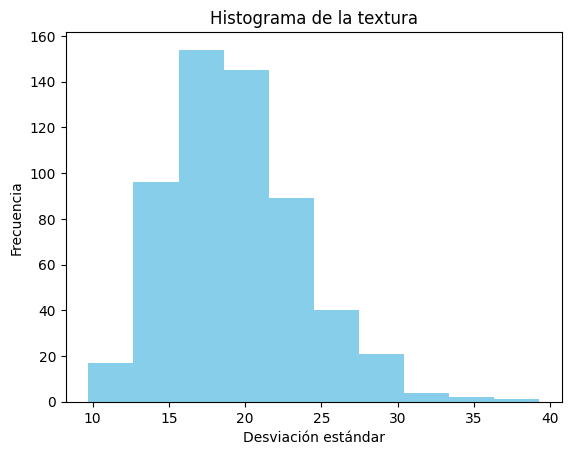
\includegraphics[width=0.6\textwidth]{images/histograma-textura.png}
    \caption{Histograma de la textura media basado en la frecuencia y la desviación estándar}
    \label{fig:histograma-textura}
\end{figure}

\newpage

\textbf{Visualización de un diagrama de dispersión}

\begin{figure}[H]
	\centering
	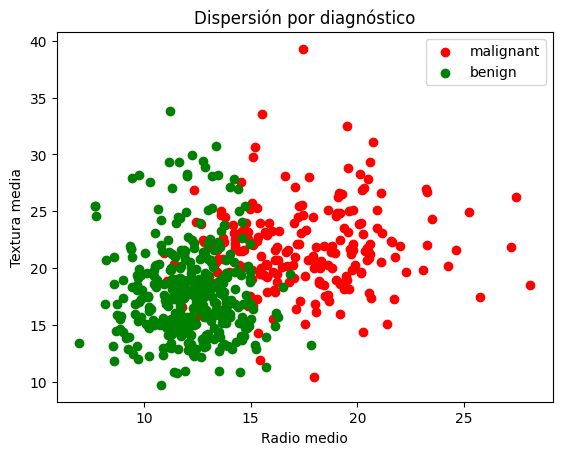
\includegraphics[width=0.6\textwidth]{images/dispersion-diagnostico.png}
	\caption{Diagrama de dispersión por diagnóstico que relaciona la textura media y el radio medio}
	\label{fig:dispersion-diagnostico}
\end{figure}

\textbf{Visualización de un diagrama de barras}

\begin{figure}[H]
	\centering
	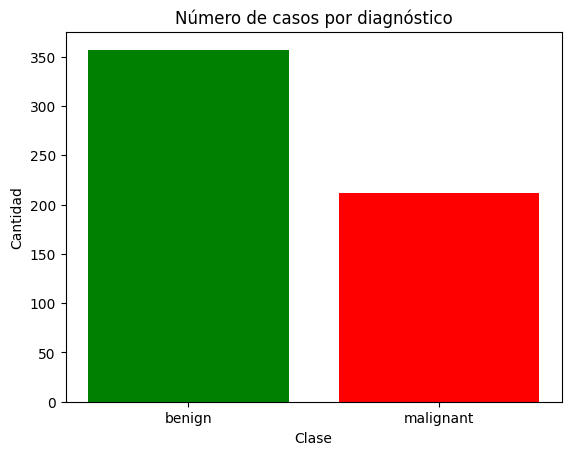
\includegraphics[width=0.6\textwidth]{images/numero-casos-diagnostico.png}
	\caption{Diagrama de barras del número de casos por diagnóstico (tumores benignos y malignos)}
	\label{fig:numero-casos-diagnostico}
\end{figure}

\textbf{Visualización de dos diagramas de líneas}

\begin{figure}[H]
	\centering
	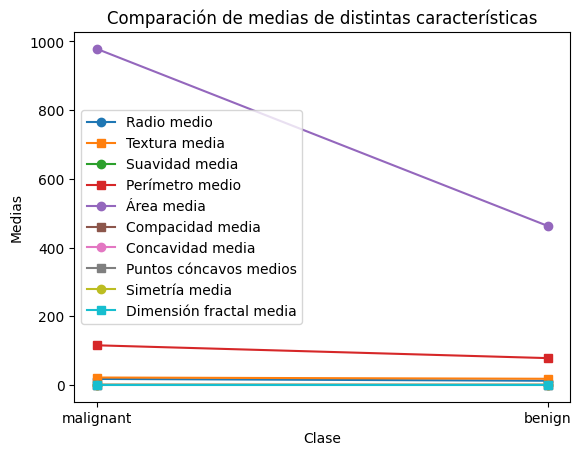
\includegraphics[width=0.6\textwidth]{images/comparacion-medias-caracteristicas-v1.png}
	\caption{Gráfico de la comparación de medias de distintas características (versión 1)}
	\label{fig:comparacion-medias-v1}
\end{figure}

\begin{figure}[H]
	\centering
	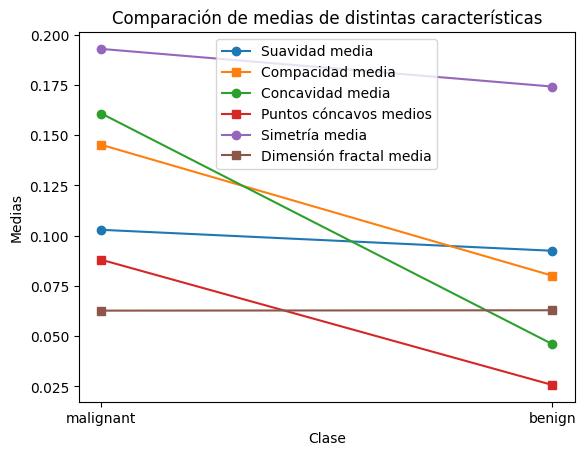
\includegraphics[width=0.6\textwidth]{images/comparacion-medias-caracteristicas-v2.png}
	\caption{Gráfico de la comparación de medias de distintas características (versión 2)}
	\label{fig:comparacion-medias-v2}
\end{figure}

\newpage

\textbf{Visualización de un diagrama de cajas}

\begin{figure}[H]
	\centering
	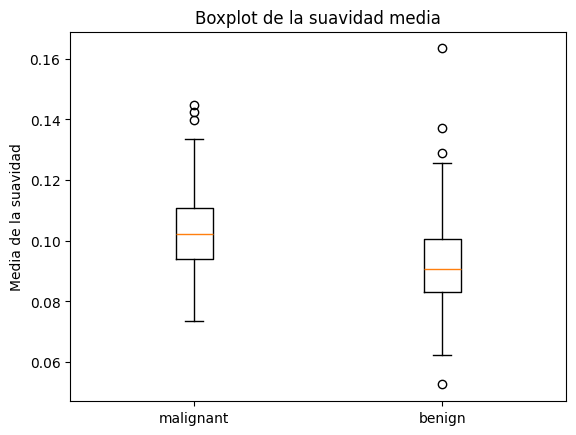
\includegraphics[width=0.6\textwidth]{images/boxplot-suavidad.png}
	\caption{Diagrama de cajas de la suavidad media}
	\label{fig:boxplot-suavidad}
\end{figure}



\textbf{Cálculo de precisión y matriz de confusión}

\begin{itemize}
    \item \textbf{Precisión del modelo:} 0.9473684210526315
    \item \textbf{Matriz de confusión:} \\
    \begin{itemize}
        \item\textbf{Eje X:} predicción\\
        \item\textbf{Eje Y:} verdadero\\
    \end{itemize}
\end{itemize}

\begin{figure}[H]
	\centering
	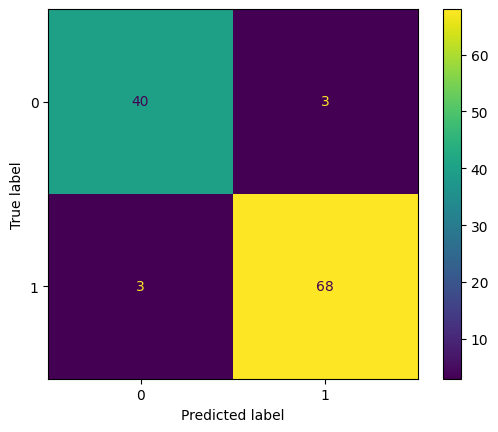
\includegraphics[width=0.45\textwidth]{images/confusion_matrix.png}
	\caption{Matriz de confusión del modelo}
	\label{fig:confusion_matrix}
\end{figure}
  


\section{Discusión}
{A continuación se van a discutir los siguientes apartados de los resultados: }

\subsection{Obtención de datos en "dataframes" con Pandas}
{Se pueden observar cuatro tablas diferentes, cada una una mostrando sus respectivos datos. En este caso nos vamos a centrar en la cuarta, la referida a agrupación por diagnóstico, ya que en esta, es posible establecer una comparación entre los dos posibles diagnósticos de una manera natural.}\\
{En dicha tabla se comparan las medias de características entre los diagnósticos benigno y maligno. Si nos fijamos en las características mostradas, podemos observar que las que tienen mayores medias pertenecen al diagnóstico maligno.}\\
\textbf{Referencia a la tabla (}\ref{tab:tabla4}).

\subsection{Visualización de un histograma}
{En el histograma anteriormente representado se visualiza la textura media, la cual está basada en la desviación estándar, asociada con su frecuencia. Vemos que la mayoría de las texturas se concentran en una desviación típica de entre 15 y 25, alcanzando un pico de frecuencia de 153 aproximadamente.} \\
\textbf{Referencia al histograma (}\ref{fig:histograma-textura}).

\subsection{Visualización de un diagrama de dispersión}
{En el diagrama de dispersión observado se clasifican las clases dependiendo del radio medio y de la textura media. Analizándolo, podemos observar que, cuanto mayor es el radio, más posibilidades hay de que el tumor sea maligno. En concreto, a partir del umbral del 15, la mayoría de los casos detectados son malignos, mientras que en la textura media se puede contemplar una superioridad benigna en valores menores a 15.}\\
\textbf{Referencia al diagrama de dispersión }(\ref{fig:dispersion-diagnostico}).

\subsection{Visualización de un diagrama de barras}
{Como se puede observar en este diagrama, de los 569 casos estudiados, hay una clara superioridad en los casos benignos frente a los que son malignos, de unos 150 de diferencia aproximadamente.\\}
\textbf{Referencia al diagrama de barras }(\ref{fig:numero-casos-diagnostico}).

\subsection{Visualización de dos diagramas de líneas}
{En este caso se han sacado dos diagramas, y esto es debido a que, como se puede observar en el primero, la característica de la media del área, al tener valores tan elevados, dificultaba mucho la visualización e interpretación del resto de características, por lo que se optó por suprimir esta. Tras hacerlo, comprobamos que volvía a pasar con otras dos, textura y perímetro.}\\
\textbf{Referencia al primer gráfico de líneas }(\ref{fig:comparacion-medias-v1}). \\
\\ {Habiendo suprimido las características mencionadas, nos quedamos con el segundo gráfico. En este, podemos observar dos tipos de casos: que las medias sean mayores en los diagnósticos benignos, o que, por el contrario, lo sean en los malignos. El primer caso corresponde únicamente a la dimensión fractal, mientras que el resto, como se mencionó anteriormente, son más altas en los casos malignos que en los benignos.}\\
\textbf{Referencia al segundo gráfico de líneas }(\ref{fig:comparacion-medias-v2}).

\subsection{Visualización de un diagrama de cajas} 

{En el diagrama de cajas podemos observar que la caja de los diagnósticos malignos está más elevada que la caja de los benignos, por lo tanto, podemos deducir que los malignos tienen una suavidad media superior.\\
También, observamos que la caja y los bigotes de los benignos son más largos que la de los malignos. Esto quiere decir que hay mayor variabilidad de la suavidad media en los diagnósticos benignos que en los malignos.\\
Por último, cabe destacar los puntos exteriores (outliers). En el diagnóstico maligno sólo hay valores atípicos a la alza (muy juntos), mientras que, en el benigno, hay más valores a la alza (con clara separación entre ellos, sobre todo el más extremo), pero también existe un valor a la baja.}
\\\textbf{Referencia a el diagrama de cajas }(\ref{fig:boxplot-suavidad}).


\subsection{Cálculo de precisión y matriz de confusión}

{Podemos observar el alto nivel de precisión del modelo (94,7\%). Eso indica que, en la mayoría de los casos, el modelo acertará en la predicción. Esto lo podemos ejemplificar de una manera más visual con una matriz de confusión, en la cual, podemos observar que de los 114 diagnósticos que realiza: 108 los clasifica correctamente (verdaderos positivos: 68 y negativos: 40) y que clasifica erróneamente por igual los otros 6 casos (falsos positivos: 3 y negativos: 3).}
\\\textbf{Referencia a la matriz de confusión }(\ref{fig:confusion_matrix}).

\section{Uso de IA generativa}

{En esta práctica se ha consultado \textbf{Gemini} para comprender la existencia de puntos fuera del diagrama de cajas (box plot), teniendo como resultado una explicación sobre la existencia de los datos atípicos (outliers). \\También se ha usado para consultas referidas al uso de \textbf{LaTeX}, como por ejemplo:}

\begin{itemize}
  \item Escribir: "\&".
  \item Configuración y dimensión de las imágenes usadas.
  \item Espaciado y sangría de los textos.
  \item Saltos de línea.
\end{itemize}

\section{Conclusiones}
{Para concluir, se puede decir con seguridad que este conjunto de datos tiene un rendimiento excelente, teniendo este una precisión envidiable del 94,73\%, siendo así todas las gráficas y resultados proporcionados muy fiables. Respecto a la interpretabilidad, sentimos que podría haber sido mejor si los datos hubiesen sido normalizados con anterioridad, estando en un rango de 0 a 1, por ejemplo. Aun así, habiendo manipulado los datos y tras el análisis las interpretaciones, se observa que el número de casos benignos supera con diferencia al de los malignos, y que, por lo general, cuanto mayor es la media de una característica, mayor es la probabilidad de que dicho diagnóstico sea maligno.}
    
\end{document}
